
\section{Buffered Read}\label{sec:conn:buf_read}

The idea of a buffered read protocol is to have a ring-buffer at the sender from which the receiver fetches the messages using
RDMA reads. There are multiple different ways to implement such a protocol, with the main variations being in, how to notify
the receiver of new messages, where to transfer them to, and how to acknowledge to the sender that a message has been processed.

\paragraph{} We decided to focus on an implementation which gives us a \emph{Passive Sender} and allows for 
\emph{Variable Message Sizes}. We decided to stick with the basic interface defined in Section~\ref{sec:protocols}. This 
results in a system with two ring-buffers, illustrated in Figure~\ref{fig:buf_read_struct}.

\begin{figure}[!ht]
\centering
\begin{subfigure}[b]{0.49\textwidth}
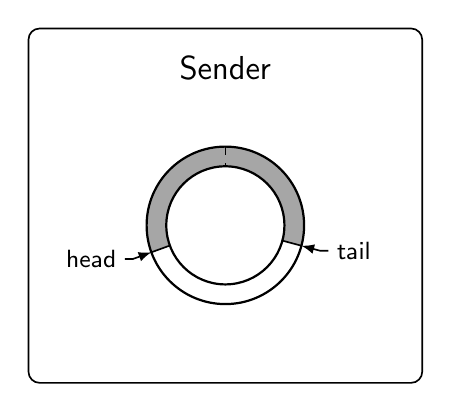
\begin{tikzpicture}[>=latex,font=\sffamily,semithick,scale=1]
    \draw[rounded corners] (-2.5, -2) rectangle (2.5, 2.5) {};
    \node[align=center] at (0, 2) {\large Sender};

    \fill [black!35] (0,0) -- (200:1) arc [end angle=-15, start angle=200, radius=1] -- cycle;

    \draw [thick] (0,0) circle (1cm);

    \draw[dashed] (90:1) -- (0:0);
    \draw (200:1) -- (0:0);
    \draw (-15:1) -- (0:0);
    \node [circle,thick,fill=white,draw=black,align=center,minimum size=1.5cm] at (0,0) {};


    \draw [<-,black] (200:1) -- (200:1.25) -- +(-.1,0)
      node [black,left,inner xsep=.1cm] (Head) {\small \code{head}};
    \draw [<-,black] (-15:1) -- (-15:1.25) -- +(.1,0)
      node [black,right,inner xsep=.1cm] (Tail) {\small \code{tail}};
\end{tikzpicture}
\end{subfigure}
\begin{subfigure}[b]{0.49\textwidth}
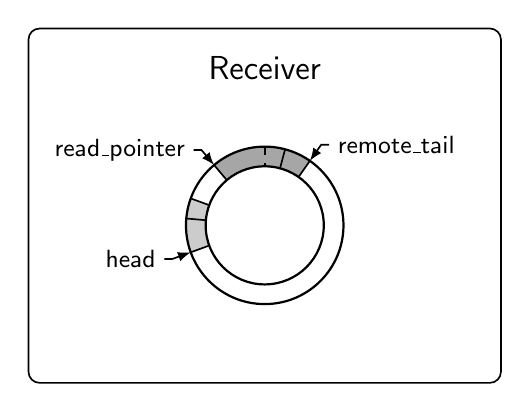
\begin{tikzpicture}[>=latex,font=\sffamily,semithick,scale=1]
    \draw[rounded corners] (-3, -2) rectangle (3, 2.5) {};
    \node[align=center] at (0, 2) {\large Receiver};

    \fill [black!35] (0,0) -- (130:1) arc [end angle=55, start angle=130, radius=1] -- cycle;

    \fill [black!20] (0,0) -- (200:1) arc [end angle=160, start angle=200, radius=1] -- cycle;
    \draw [thick] (0,0) circle (1cm);

    \draw[dashed] (90:1) -- (0:0);
    \draw (200:1) -- (0:0);
    \draw (175:1) -- (0:0);
    \draw (160:1) -- (0:0);

    \draw (130:1) -- (0:0);
    \draw (75:1) -- (0:0);
    \draw (55:1) -- (0:0);
    \node [circle,thick,fill=white,draw=black,align=center,minimum size=1.5cm] at (0,0) {};


    \draw [<-,black] (130:1) -- (130:1.25) -- +(-.1,0)
      node [black,left,inner xsep=.1cm] (rptr) {\small \code{read\_pointer}};
    \draw [<-,black] (200:1) -- (200:1.25) -- +(-.1,0)
      node [black,left,inner xsep=.1cm] (Head) {\small \code{head}};
    \draw [<-,black] (55:1) -- (55:1.25) -- +(.1,0)
      node [black,right,inner xsep=.1cm] (Tail) {\small \code{remote\_tail}};
\end{tikzpicture}
\end{subfigure}
\caption{Structure of the buffered read connection}
\label{fig:buf_read_struct}
\end{figure}

\subsubsection{Protocol}
As mentioned the sender of our buffered read connection is entirely passive, that means after the connection setup the sending
CPU does not issue any RDMA operations. The only thing it needs to do to send is to check its head if there is enough space,
copy the message to its tail, and update the tail offset.  It also prepends the message size when  writing. 

The head is completely managed by the receiver and the tail pointer needs to be accessible to it. That means for the sender,
transmitting a message does only involve copying it to its local memory. This results in
a very low sending overhead.

\paragraph{} A completely passive sender means the receiver has to do the heavy lifting. The receiver manages three different pointers: 
the \code{read\_pointer} which marks the beginning of the next message to receive, the \code{remote\_tail}, which is a cache of
the senders tail and marks the end of the transmitted buffer section, and the \code{head} which marks the beginning of 
the earliest not freed message.

\paragraph{} Receiving a message now involves the following. We first check if there are already transmitted messages that 
we have not received yet. Meaning the \code{read\_pointer} is not equal to the \code{remote\_tail}. If so, we can simply 
return the next message with the length at the beginning of the buffer and update the \code{read\_pointer}.

If there are no transmitted messages to return, the receiver updates the \code{remote\_tail} with an RDMA read. If the remote
tail has not updated, it retries until it has. With the updated tail the receiver issues an RDMA read for the whole buffer 
section between the read pointer and the updated tail. It then returns the next message in the newly transmitted section.

This gives us an interesting characteristic of most receives being very cheap, while some are very expensive as they need to 
perform a large read. We did not implement preemptive issuing of reads which could reduce this effect and improve performance
significantly.

\paragraph{} To keep track of the freed buffers at the receiver we use the same linked list structure we used in the buffered
write connection. This allows us to update the \code{head} accordingly when freeing messages out of order and freeing will
occasionally update the remote head using an RDMA write operation.

\paragraph{} For both ring-buffers we use the same \emph{"Magic Buffer"} trick introduced in Section~\ref{sec:conn:buf_write} to 
allow us to wrap around the end of the buffer.

\subsection{Feature Analysis}
The Buffered Read connection is probably the most different protocol compared to the other connections we evaluate in this
thesis. Our design ended up very similar to a \emph{Flow Structure}~\cite{sharma2020design}.

\paragraph{} The protocol results in a completely \emph{Passive Sender} and achieves effective memory usage through \emph{Variable Message Sizes}.
The buffered read protocol does not achieve \emph{True Zero-Copy} capabilities, as the sender always needs to copy the 
message into the send buffer and the receiver will most likely need to copy the message out of the receive buffer. It also
has the same \emph{Blocking} behaviour as the buffered write protocol.


\paragraph{} For future work it would also be interesting to implement a system where multiple threads can write to and receive 
from a single  connection by atomically updating head or tail pointers, or we could explore the possibilities to share send or
receive buffers using atomic operations. The current implementation, however, does not provide any kind of \emph{Resource Sharing}
